%%%%%%%%%%%%%%%%%%%%%%%%%%%%%%%%%%%%%%%%%%%%%%%%%%%%%%%%%%%%%%%%%%%%%%%%%%%
%                                                                         %
%      This file is part of the 'openLilyLib' library.                    %
%                                ===========                              %
%                                                                         %
%              https://github.com/lilyglyphs/openLilyLib                  %
%                                                                         %
%  Copyright 2012-13 by Urs Liska, lilyglyphs@ursliska.de                 %
%                                                                         %
%  'openLilyLib' is free software: you can redistribute it and/or modify  %
%  it under the terms of the GNU General Public License as published by   %
%  the Free Software Foundation, either version 3 of the License, or      %
%  (at your option) any later version.                                    %
%                                                                         %
%  This program is distributed in the hope that it will be useful,        %
%  but WITHOUT ANY WARRANTY; without even the implied warranty of         %
%  MERCHANTABILITY or FITNESS FOR A PARTICULAR PURPOSE. See the           %
%  GNU General Public License for more details.                           %
%                                                                         %
%  You should have received a copy of the GNU General Public License      %
%  along with this program.  If not, see <http://www.gnu.org/licenses/>.  %
%                                                                         %
%%%%%%%%%%%%%%%%%%%%%%%%%%%%%%%%%%%%%%%%%%%%%%%%%%%%%%%%%%%%%%%%%%%%%%%%%%%

\documentclass[../../LilyPond-Tutorials]{subfiles}

\usepackage{fancybox}
\RequirePackage{multicol}
\RequirePackage{tabularx}
\RequirePackage{fancyvrb}

\begin{document}
\parttitle[Urs Liska]{Editing Musical Documents as Plain Text}
\begin{authorAbstract}{Urs Liska}
Abstract
\end{authorAbstract}

\chapter*{Introduction}
\label{chap:pt_introduction}
This paper discusses an approach to authoring musical documents%
\footnote{i.\,e.\ scores and texts about music}
that is based on editing \emph{plain text files} instead of using graphical \textsc{wysiwyg} software%
\footnote{What You See Is What You Get---such programs provide an editing environment where the document is displayed identically to the way it will be printed.}.
The described concepts, tools, and workflows have significantly changed my life as a document author, and I  wholeheartedly endorse them because I strongly believe in their unique and substantial advantages.

The plain text approach is practically non-existent in the humanist disciplines or in the music business, while being de facto standard in many natural and computer sciences.
Working with plain text based tools indeed requires a certain shift in mind-set for people who aren't already familiar with the corresponding working paradigms.
And it can't be denied that the learning curve is considerable.
But this investment is absolutely justified because on the long run it greatly benefits productivity and offers potentials unimaginable otherwise.
Reading and writing music, playing an instrument, investigating a manuscript source---all this involves a very long and intense learning curve, and we mastered them as a matter of course in order to become the professionals we are.
So why be afraid learning something new?

This paper is focused on scholarly and collaborative workflows, particularly preparing musical editions for publication, because that's my cup or tea.
But most of it will equally apply to creating musical scores or texts about music that have a certain level of complexity.
The described concepts will also prove useful for people who have to deal repeatedly with similar document types, such as presentations, teaching/exam materials, music examples etc.
However I will \emph{not} cover workflows that mainly depend on instant results but don't care about structure or output quality, such as just-in-time arranging or the like.
For such applications plain text tools may not be the appropriate choice.

If you expect an in-depth description or even a guide how to use the mentioned tools you might be disappointed because that's not the intention of this document.
What I hope to give you is a sense of the power that text based approaches can give you.
For this I will discuss the topics mostly from a rather elevated point of view, keeping your exposure to concrete examples at a minimum%
\footnote{with the exception of some intentionally spectacular examples}.
At the end of the text I will direct you to more extensive material that is suitable to get you more intimately acquainted with the relevant concepts and that may actually aid you getting your feet wet with editing plain text files.

The software packages I will introduce you to on the following pages are:
\begin{itemize*}
\item \emph{LilyPond} -- the program that lets you engrave beautiful scores
\item \emph{Git} -- the versioning system that keeps your work under control
\item \emph{\LaTeX} -- the professional typesetting engine for text documents
\end{itemize*}

\chapter{Plain Text Format}
\label{chap:pt_plain-text-format}
Who on earth would voluntarily enter music as a text file?
Aren't these people just nerds who think that only what hurts can be good?
Isn't it \emph{natural} to edit musical scores within a graphical user interface?

Well, when computers became more powerful it was an inevitable development to provide increasingly powerful graphical user interfaces, allowing users to edit any visual aspects of a document visually with a mouse or other pointing device.
This is obviously quick, effective and easy approach.
But considered seriously and open-minded there are lots of reasons why it \emph{is} a good idea to edit and store documents in text files.
Text based work avoids several fundamental problems that other approaches share, and it opens up a whole range of advanced options not imaginable otherwise.
And it is good to know that by now there are editors available that significantly assist you in dealing with text files.

To start getting into the topic I will consider a number of features of working with plain text files.
Mostly this applies equally to text documents and scores, although the emphasis of this paper clearly is on musical engraving.

\section{Transparency and Control}
\label{sec:pt_transparency-and-control}
Have you ever wondered how your notation program internally manages the contents you entered?
Not as a mental exercise but because you had the impression it maliciously made fun of you?
One of the reasons I turned my back on graphical notation programs was my frustration with being completely at the mercy of the software with regard to my personal layout decisions.
I can't recall (and actually don't want to) how often I ran through the loop of
\begin{inparaenum}[1.)]
\item entering music,
\item moving items around ,
\item applying some manual tweaks like flipping stems, breaking beams, suppressing or parenthesizing cautionary accidentals,
\item hitting “Update Layout” and finally
\item tearing my hair out because at least one third of my manual settings mysteriously vanished.
\end{inparaenum}

Maybe my judgment isn't fair because it is based on very outdated software.
Maybe things have improved a lot, but the fundamental fault is still valid: 
I am at the mercy of the software and can't see or control how it represents the content internally.

A friend finally stopped using (a later version of) the same graphical program when he fixed one missing accidental in a score he had earlier tweaked to perfection---and this accidental caused the whole layout to break irreversibly.

Besides this risk of losing work I also can't usually tell how the program interprets my displacements applied through a pointing device.
Are they interpreted as offsets relative to some point on the page, or relative to the original decisions of the program?
Are they measured in fixed units or with some proportional factor?
None of that would be wrong, but I just don't know about it, and it \emph{does} make a difference if the layout changes afterwards for any reason.

\medskip
\todo{Example how this applies to text documents}

\medskip
If I edit a plain text file instead I'm completely in control over all these issues.
If I tell the program to break a beam or to draw a slur above the note it is explicitely and reproducibly defined and readable by anybody.
There is nothing hidden in “settings” dialogs or even unreadably buried somewhere in the file as the result of dragging something with the mouse.
If I manage to break something (which of course happens) I can review what I did, compare to the last working version%
\footnote{See the “version control” \fref{chap:pt_version-control}}
and understand and fix the issue.
With a graphical program my only resort is to “undo” and hope this will fix it \dots

There is a price for this, namely having to enter code by hand and learning how to do that, but it is very rewarding on the long run.
And being in control just \emph{feels} better \dots

\section{Content, Meaning and Appearance}
\label{sec:pt_separation-content-meaning-appearance}
Through the overwhelming presence of \textsc{wysiwyg} applications we have got used to the impression that the \emph{visual appearance} of a document is identical to its \emph{content}.
But this is actually a quite shortsighted assumption.

If you look at that text document:

\begin{center}
\noindent\shadowbox{\parbox{.8\textwidth}{%
\Large \textbf{\textsf{My new chapter}}

\medskip
\normalsize \textbf{\textsf{With a section}}

\medskip
\small This is the \textbf{\textsf{continuous}} text with some \textbf{\textsf{emphasized}} words.}
}\end{center}

\noindent you will notice that there are several parts formatted in sans-serif bold face of different sizes.
You may guess that the author has applied several style sheets to get this appearance, but to verify it you'd actually have to select the texts and look into the corresponding dialogs or toolbox elements.
Only then you can see whether the author manually formatted the text, applied paragraph styles or character styles.
He may even have applied character instead of paragraph styles to format the headings.

The corresponding \LaTeX{} source file would look like:

\begin{lstlisting}[language={[LaTeX]TeX}]
\documentclass{article}
\newcommand{\terminus}{\textbf{\textsf{#1}}}
\begin{document}
    \chapter{My new chapter}
    \section{with a section}
    This is the \terminus{continuous} text with
    some \textbf{\textsf{emphasized}} words.
\end{document}
\end{lstlisting}

While this may look complicated on first sight it actually is much clearer because it distinctly shows you the content and the author's intentions.
The \cmd{documentclass} is something like a document template, but much more powerful%
\footnote{See the \LaTeX{} chapter \fref{chap:pt_latex}}.
\cmd{terminus} is defined as a character style applying bold (“\dots bf” for BoldFace) and sans-serif (“\dots sf” for Sans-Serif) to its content (“\#1”).
Inside the document body (enclosed by the \cmd{begin} and \cmd{end} statements) you can see the \emph{content} along with \emph{semantic markup}.
The two headings use explicit sectioning commands which are (for now) equivalent to paragraph styles.
The two bold words in the text line are formatted differently: 
the first one  is enclosed by our \cmd{terminus\{\}} character style while the second one is manually formatted as bold and sans-serif.
This mixture of formatting techniques is highly disadvised and only used for the sake of the example.
But you may notice that in the plain text file this “problem” is immediately obvious while the graphical program actually hides away such inconsistencies.

\medskip
If we think about musical scores we have to come to a very similar conclusion.
I began this chapter with the rhethorical pretention that it is “natural” to edit a score in a graphical way.
But in fact that's not entirely true because a score isn't a graphical object like a painting
but rather a graphical \emph{representation} of the musical \emph{content}.

If you consider the following minimal score and its (complete) LilyPond input file:
\begin{multicols}{2}
\vfill
\begin{musicExampleNonFloat}
\begin{quote}
\lilypondSFE{examples/minimal-score}
\end{quote}
\end{musicExampleNonFloat}
\vfill
\columnbreak

\begin{centering}
\begin{lstlisting}
{
  \time 3/4
  \key es \major
  \clef treble
  es'2.
}
\end{lstlisting}
\end{centering}
\end{multicols}

\noindent you can see that the source on the right side completely defines the \emph{musical content} of the score:
a time signature, a key definition, a clef, and a single note with duration.
Of course the page layout is also an inseparable part of the score document, but on a conceptual level it is completely separate from the musical content.
Without going into more detail here you should note that in LilyPond's plain text file you have complete control over the separation of content, meaning and appearance.
While this at first may seem somewhat abstract it is actually a very important point when it comes to preparing different output from one source%
\footnote{See “single-source publishing” section \fref{sec:pt_single-source-publishing}}.

\section{Readability and Stability of Text and Binary Files}
\label{sec:pt_readability-stability}
In the previous section you have seen examples of plain text files for a text and a score document.
OK, I admit that it takes some time getting used to filtering out the markup commands in a text file mentally.
But I can't emphasize enough that you actually \emph{can read} that file \emph{at all}.

Does this bold statement surprise you?
Don't you think that you can immediately conceive the content of the graphical score, much faster and easier than the source file that you first have to read and interpret?
Well, then you are again exchanging the real document file and the graphical representation the graphical programs expose to you.

Please take the time and have a look at \todo{prepare “listings”, put them in appendix and add link to them}.
That's what the file contents from the previous examples actually look like.
After skimming through the Word\texttrademark, OpenOffice\texttrademark, Finale\texttrademark{} and Sibelius\texttrademark{} files you should reconsider the “overly complex” \emph{source code listings} of the previous section.
Now you'll probably see why I emphasize that you can \emph{read} \LaTeX{} and LilyPond files, isn't it?
You may have noticed that both Word\texttrademark{} and OpenOffice\texttrademark{} also have an alternative file format that is stored in “plain \textsc{xml}”.
While a human actually \emph{can} read these files the actual content is very deeply buried inside them and practically inaccessible to the human eye.
	
The fact that plain text files are human readable has two major implications:

\paragraph{Recovery after file corruption}
There are several ways that can make a file unusable, the most common being accidental deletion, a general disk failure or the crash of a program leading to an inconsistent state of the file (the latter fortunately becoming increasingly rare nowadays).
Usually such files can be partially retrieved with special tools, but the picky thing is the “partially”.
If you have a binary file that can only be read by its original program the whole file is now unusable, even if the corrupted portion is very small.
From a corrupted plain text file on the other hand you will be able to retrieve everything \emph{as content} that is still there at all.
And with some luck you may even guess the missing pieces.
Sometimes it will still be more efficient to start again from scratch, but depending on the nature of your project this characteristic of plain text files may actually be a life-saver.

\paragraph{Restoring “ancient” files}
As programs mature they modify their file formats.
Usually programs can still open the files from older program versions, but that isn't an endless option.
With the majority of programs you would need to have some older version to be able to open “ancient” files.
This may actually be a monetary factor---and with some “luck” there doesn't even exist a version that runs on your current operating system.

This may also happen with programs that store their data in plain text files.
But as the file format is usually much better documented it is more likely that you will find a conversion option still available.
And if everything fails and you have a file but no dedicated editor you still have the plain text and free access to it.

\section{Editor Independence}
\label{sec:pt_editor-independence}
Plain text workflows separate the tasks of editing, processing and displaying documents.
This way you are not restricted to \emph{the one} application the (commercial) vendor imposes on you, but you are free to chose any editing environment you like, consider appropriate or just feel comfortable with.
There are programs that try to integrate all parts of a workflow, just like the \textsc{wysiwyg} tools do---but it is your free choice to use them or not.

You can even edit a project with different tools at a time.
For example it might be handy to be able to edit a document with any text editor on your smartphone, or just going to a public internet access point and send yourself an email with a sketch---both of which you would then process to a pdf document when you are home again.

Another interesting application is the use of plain text as input to web forms.
Many web forms, e.\,g.\ in forums, allow you to enter your posts in \emph{Markdown}%
\footnote{\url{http://daringfireball.net/projects/markdown/}},
a minimalist plain text language, and convert them to formatted \textsc{html}.
And by now you can even enter LilyPond code that will be rendered as music examples in Wikipedia entries.

\section{Programmability}
\label{sec:pt_programmability}
Plain text files can be edited not only by any text editor but by \emph{anything} that can edit text files---which makes it accessible to about any programming language you may think of.
You are not restricted to any scripting interface the vendor graciously provides you, but you can apply any imaginable operations with your source files: 
analyze them,
process them,
or even computationally generate them from scratch.

I you have never programmed and don't intend to learn it you may think that's a rather unimportant feature.
But this isn't true at all.
A project you are working with can hire (or have) someone with that ability, so the whole project can benefit enormously from the versatility this offers---without the individual members needing to see any line of programming code.

There are many possible applications, from applying contrapuntal operations or algorithmic composition up to managing music examples in a database.
For example I'm currently working on the infrastructure for a large orchestral score where those who enter the music only work on small segments of the instrumental parts.
The full score (which is initially filled with rests) will automagically build itself and use whatever segments have already been entered.

\section{Compiling Files vs.\ Instant Feedback}
\label{sec:pt_compiling-instant}
One thing the average \textsc{wysiwyg} user needs to get used to is \emph{not} to get instant feedback.
Graphical programs immediately display any updates in their graphical user interface, while the text files first have to be \emph{compiled} before you can see the results of your modification.

While this may seem cumbersome, it actually isn't a problem but an inherent advantage, and a big one!
Other than the graphical program the compiler can first read the input file, get a solid internal representation of the content and structure, and finally take its time to produce the best possible layout for the given content.
It can judge the implication of a modification for the whole document and rethink the layout completely.
The problems graphical programs are encountering are immediately visible when you (for example) try to move a figure in a 250 pages text document with 80 figures, or when you insert some music in the middle of a longer score---tasks that don't upset text based programs at all.

As a logical result from this different approach text based programs (I'm speaking of LilyPond and \LaTeX{} in particular) produce \emph{default output} of significantly superior quality than their graphical counterparts.
While it is obviously possible to produce publication quality output with Finale\texttrademark{} or Sibelius\texttrademark{} (but not with Word\texttrademark{} or OpenOffice\texttrademark) the default output of Lilypond is practically always \emph{readable} and \emph{usable} without any further intervention.
As a rule of thumb I'd say that you can use LilyPond scores (and \LaTeX{} documents) without bothering about layout details as long as you don't want to publish them.
This is a significant improvement for the development process of documents and editions as you can work on the real \emph{content} up to the final stage of print preparation.

Look at the following example of a rather complex score%
\footnote{Arnold Schönberg: Excerpt from “Gethsemane” (fragment).
\todo{ask Larry Schoenberg for permission}
First published in: Arnold Schönberg. Sämtliche Werke \dots
}:

\begin{musicExampleNonFloat}
\lilypondmfe[examples/gethsemane]
\end{musicExampleNonFloat}

\noindent and note that there isn't a single manual intervention beyond assigning the music to the right voice contexts.
It is really amazing how LilyPond manages to do most things immediately right.
While the score isn't perfect to publication quality there is \emph{nothing} that hampers reading the music when placed on the music stand.

Now have a look at the following example of a rather complex score%
\footnote{Arnold Schönberg: Excerpt from: “Nie ward ich, Herrin, müd” | Nr. 4 aus “6 Orchesterlieder" | für Gesang und Orchester | op. 8/1, \copyright{} 1911 by Universal Edition A.\,G., Wien/UE 3041, \href{http://www.universaledition.com/}{www.universaledition.com} [permission granted for use in this tutorial. You may redistribute the document provided you keep this copyright notice and the hyperlink in place]}
that LilyPond did \emph{not} manage to engrave perfectly without assistance:

\begin{musicExampleNonFloat}
\lilypondSFE{examples/schoenberg-opus-8-4}
\end{musicExampleNonFloat}

Please note that there is no single manual tweak to that engraving.
I just entered the music and assigned the right voice contexts to it.
Of course this is far from perfect, and the LilyPond developers would surely take this example as a source of inspiration for improvements of the engraving engine.
But if you excuse the long phrasing slur from m.\,1 throughout 3 (which I judge no automated engraving system would be able to get right by itself) you will notice that the engraving is completely readable---you could put it on the music stand and play from it right away (which I can confirm from practical experience \dots).

If you compare that to the attempt one of the two “big players” took at the same measures (with the same task description: entering music, assign voices correctly, no further manual tweaks), you will understand what I mean \dots

\begin{musicExampleNonFloat}
    \musicSFE[trim=2.6cm 21.5cm 1.3cm 2.9cm, clip]{examples/schoenberg-opus-8-4-finale}
\end{musicExampleNonFloat}


There are a few more features about working with text files that I'll write about in the LilyPond \fref{chap:pt_lilypond}, namely the potentials of using \emph{variables}, of being able to \emph{include} files and design sophisticated cascading set-ups, and finally of \emph{commenting} and \emph{documenting} source files.
But first let's take the time to learn about what is maybe the single most important feature of plain text files: their accessibility to \emph{version control}.

\chapter{Version Control}
\label{chap:pt_version-control}

\emph{Version control} is a concept I had heard of long ago, and I assumed it was one of the tools belonging to software development in general.
But realizing that it can very well be used by musicians and musicologists was a revelation that made me completely revise my working methods last year.
It actually \emph{changed my life} as a document author, and I can't imagine how I could ever have existed without \dots

As a first approximation you may understand version control as an infinitely flexible implementation of \emph{undo/redo} mechanisms.
Versioning stores the complete development history of your document or project and lets you investigate \emph{any} state it has ever been in over time.
Furthermore it lets you roll back (or reapply) \emph{any individual} change you have applied at any time, not necessarily in (reverse) chronological but in arbitrary order.

Suppose two weeks ago you reworked a chapter of your book and now you realize that someone else has just now published exactly the same insights---you need to remove these changes and try to get the chapter into the state it had been before.
With a traditional toolchain you would be lucky to have a version of that state at hand, either as a backup file or printed on paper.
With the backup file you may roll back your work to that state---but of course you lose all work done afterwards.
Or you could put the (digital or printed) backup and the current version side by side and manually emend the changes you applied.
Both solutions are cumbersome, error prone, and they rely on the---random---existence of a backup of exactly the desired state.

With a document under version control on the other hand you may identify the exact changeset that you want to undo and just revert these changes---and leave everything done before or after the way it is.
It may not be obvious to you, but this can easily span decades, programs, and even operating systems' lifecycles---because it works on plain text files as seen in the previous chapter.
You think that's cool? I can tell you it \emph{is}!
And this is just the surface -- we'll later deal with other, maybe even more important aspects of versioning.

\section{Basics of Version Control}
\label{sec:pt_basics-version-control}
The fundament all this is built upon is the line-by-line comparison of the complete project directory that the versioning program performs when you “save” your project%
\footnote{The actual terminology is different but I'll try to use familiar terms as long as possible.}.
Of course these “lines” that are compared refer to the lines in your plain text files.
In a text document a line will usually contain one coherent entity like a sentence, a list item or the like.
In a score this might be (depending on the complexity of the material) one voice in one measure.
(Of course you can lay out your text files as you want.)
So this means that whenever you save your project the versioning software records (e.\,g.) which sentences or which measures you have modified, stores this as a \emph{changeset}, and adds this to the project history.
And you can completely decide for yourself how fine-grained you tailor such changesets:
They may envelope the work of a day, the complete revision of a chapter or a single corrected note.
But note that the first example is actually a bad one because the idea of versioning is to organize the history of a project as a series of \emph{coherent} sets of changes. 
Probably you'd rather split your day's work into snapshots like 
\begin{inparaenum}[1.)]
\item “proof-reading choir parts” 
\item “adding critical notes”
\item “reorganize directory structure”.
\end{inparaenum}
Note that this concept does work on the project directory and not on single files.
So a changeset can span a whole set of files, thus linking related work together.

Once you have saved a changeset to the project it is part of its history, and it is practically impossible to lose that work again by accident.
To achieve this you would have to apply some really advanced tools you normally never touch.
You can think of a project under version control like a bag where you put all your stuff in, while the versioning software keeps track of all changes.
Whenever you want to investigate any earlier state of your project the versioning system uses the content of the bag and its own records to bring your project directory into the form it had at that specific state.
From there you can revert, modify or reapply any changeset that doesn't create structural conflicts%
\footnote{Such a conflict would for example arise if you would try to revert changes to some lines in file that has in the meantime been deleted.}.

But you could also create a new \emph{branch} from that state.
\emph{Branching} is one more important concept of source code versioning.
You can see a branch as a “session” that is independent from other lines of work.
To use the given example (of inspecting an earlier point in project history) you might go back to a certain point, create a new branch and work in a different direction.
If you are satisfied with this new approach you can simply replace your earlier work with the new one (while not completely losing it because it's kept in the project history)---or you can decide to throw away the new attempt and switch back to the original version of your document.
A more common application of branches is to start any new work that might get your document/project into an inconsistent state in the context of a branch.
This is merged with the main line of work only later when it is finished.
An example for this would be integrating the results of a critical revision into a score---this way the main line would keep its consistent original state up to the moment when you merge in the revision in one single step.

Until now I have omitted mentioning any concrete software that does this ominous versioning.
This is because there are numerous tools in this area, but they more or less share the described concepts.
In their generic form they all are command line programs that you can tell to perform actions on your project like saving a new changeset, managing branches or inspecting dedicated states of history.
For all versioning systems there exist graphical front-ends for all major operating systems that aim to ease working with the systems.
But one has to admit that versioning systems are \emph{very} powerful tools that consequently deserve some work getting used to and some care in working with them.
You \emph{may} have heard the names \emph{CVS, Subversion, Git} or \emph{Mercurial}, but if you don't it's no problem.
They share some concepts and differ in others---but that is beyond the scope of this article and actually completely unimportant for its purpose.


\section{Collaborative Editing}
\label{sec:pt_collaborative-editing}

While all this is already very exciting we still haven't touched the most important aspect of all: the impact versioning can have on the concepts of \emph{collaborative editing}.
The ambiguity of the expression is intended---I'm talking about editing (or more generally working on/with) musical works in a collaborative and social way, and I'm talking of simultaneously editing source files.
To emphasize the potentials I will take a step back and first describe traditional ways of collaboration (“traditional” being quite relative, of course).

\medskip
The most basic way to collaborate on a project is to exchange ideas personally, by phone or by email, and have one person edit the document(s).
This way the document is guaranteed to be in a consistent state, but the workflow isn't really practical if you don't happen to share an apartment or at least an office.

The next (and quite common) way is to exchange documents by email or on data storage media like disks or \textsc{usb} devices.
You will surely have already worked that way or do it regularely.
While this \emph{may} work in simple cases (for example two collaborators and only a very small number of files) it adds complexity that can easily lead to problems:
\begin{enumerate*}
\item What do I do with a document returned by a partner?
Do I replace my original version or do I make a copy (presumably named something like “essay-revision-Michael-2009-12-04” or “essay-v003”)?
What if there are more than two people and/or numerous iterations involved?
\item How do I prevent the situation that a document is simultaneously modified by different people?
This can easily happen if my partner sends a document a second time with further modifications while I have already made changes to it.
If we're lucky and notice the conflict at all the only resort is probably to compare the files manually!
\item Working with such a system is only possible if you are dealing with a quite small number of files.
Currently I'm working on an edition project with a project directory containing more than 500 files.
It would definitely be impossible to even try to keep track of modifications of this number of files via email.
\end{enumerate*}

\medskip
The first and the last problem can be dealt with by storing the files at some shared location---in a local network or at one of the numerous providers of \emph{cloud based} storage.
This way you don't have to manage different copies of your documents, which improves the situation a lot.

\medskip
The second problem however---preventing simultaneous modifications---can't be solved reliably with this approach.
To avoid conflicts a team has to obey to strict policies that aren't always easy to enforce.
People have to “lock” files they want to edit, which is quite difficult if they aren't permanently connected to the network.
While not theoretically impossible such an approach bears an enormous inherent risk, especially with larger numbers of collaborators---and sooner or later there \emph{will} be accidents \dots

This is where \emph{version control} comes into play, and this is where we \emph{really} enter new grounds in our scholarly or artistic workflows.
Using plain text files and version control enables us to benefit from techniques and strategies that have been invented for and improved for decades in software development%
\footnote{In fact Git has been originally written to manage the development of the Linux kernel.}.
And the key concept in this regard is \emph{collaboration}.
Software is mostly developed by teams or even large communities, and version control systems have been originally designed to seamlessly manage contributions by a large number of people.
For example the Linux kernel project accounts for several hundreds of thousand “commits” by more than 10.000 contributors.

\medskip
The heart of a versioned workflow is a shared data inventory, or \emph{repository,} located on a server that is accessible by all project members%
\footnote{This could be a server on the local network or---much more common---a dedicated service provider such as GitHub (\url{https://github.com}) or Bitbucket (\url{https://www.bitbucket.org})}.
With \emph{distributed} version control (which is what I'm talking about exclusively) each contributor has a local copy of the repository on which he can work without having contact to the shared server.
There he adds his snapshots to the project history (as described earlier), and whenever it is appropriate or practical he can synchronize his work with the data on the server, downloading the new work from others, integrating this with his own work and finally uploading the local changes to the shared repository.

Earlier I wrote that version control is based on line-by-line comparison of files.
This is of even greater importance in distributed collaborative workflows, as it effectively renders file locking unnecessary.
I would like to stress that it is for example even possible that one contributor adds articulations to one hand of a piano part while another one at the same time fixes engraving shortcomings in the other hand of the same measure without any problem.
As long as the two people won't modify \emph{the same line} in the same source file, all of this synchronization will work silently without anybody really noticing it!

Of course this isn't effective because it makes conflicts \emph{unlikely}---this would actually be quite negligent.
The point is that potential conflicts can be reduced to the conflicting line(s) in the source file.
If simultaneous changes can't be reconciled because of a conflict the contributor faced with it will find markers in the text file indicating the conflicting versions.
From there he can decide individually which version to keep (or the mix them) and submit the result to the versioning system.
So while versioning can't completely prevent conflicts it significantly reduces the hassles to recover from them.

\medskip
Another feature that has become crucial to my work relies on the way versioning software records changesets.
As described earlier they keep track of file differences, and they can be inspected later.
This way I can see exactly what my partner has done to a file without even bothering to compare the files manually or visually%
\footnote{In fact I can even inspect others' changes on the go, as there exist smartphone apps for several hosting providers}.
Office programs have a feature to record changes (whatever it may be called in a given program and language).
But once I have accepted or rejected the changes this (visual) indicator has vanished while the changesets are part of the project history and therefore eternally present.

\medskip
To sum up: in a project with version control each contributor has access to and can work simultaneously on the whole data inventory, with very little risk of conflicts and a straightforward way to resolve conflicts that may eventually arise nevertheless.
This opens up quite a lot of perspectives on collaborative work that I consider very promising.
In the last chapter \fref{chap:pt_applications} I will describe some of them.

\chapter{LilyPond}
\label{chap:pt_lilypond}
When it comes to engraving musical scores my tool of choice is \emph{GNU LilyPond}%
\footnote{\url{http://www.lilypond.org}}.
Not only do I love its beautiful score output, but I really value how seamlessly and professionally I can integrate scores with (\LaTeX) text documents, and I have come to absolutely rely on the workflows and concepts based on the plain text approach that it allows.

Of course I would love to give you a thorough introduction to this amazing software but that would be quite pretentious and especially out of scope of this article.
Therefore I will keep my focus on the potentials of the text based approach, giving you just enough information to get an impression on how it would “feel” to work with it and to get the necessary foundation for the following ideas.

As you know quite well by now LilyPond works by reading in text files and processing them to engraved scores.
So one effectively \emph{has} to learn how music is represented in LilyPond's input language.
But it may be good to know that while it is actually possible to edit the text files with any plain text editor there actually \emph{are} graphical programs assisting you heavily in dealing with the text files.
Although there are a few I will only show you one.

\section{Frescobaldi}
\label{sec:pt_frescobaldi}

\textit{Frescobaldi%
\footnote{\url{http://www.frescobaldi.org}}}
is a complete editing environment that allows you to do everything you need within one interface.
In that it is quite similar to the graphical programs I have earlier dismissed as conceptually flawed.
But there is a big difference, as Frescobaldi presumably offers the best of both worlds:
it gives you the greatest possible graphical access to the editing process while in its core still being a---sophisticated---text editor.

Its main window presents itself like many programs that allow to edit textual source files of graphical documents: it is split in a \emph{text editor} and a \emph{music view} (see \fref{fig:pt_fb-main-window}).
In the music view on the right hand you see (surprise) the music.
Please note that a) Frescobaldi isn't responsible for generating the engraving in this view and b) this view doesn't have a  “live“ connection to the source but is only updated when LilyPond is run.
So you could actually call Frescobaldi a \textsc{wysiwyg} editor because what you see actually \emph{is} what you finally get---but you can't (yet) edit the score in a graphical way in this music view.
On the left side of the screen shot you can see the \emph{Quick Insert} widget, one of the tools that simplify your life by “remembering” how to insert all sorts of graphical symbols for you---but again: they won't insert them “into the score” but as text into your input file.

\begin{figure}
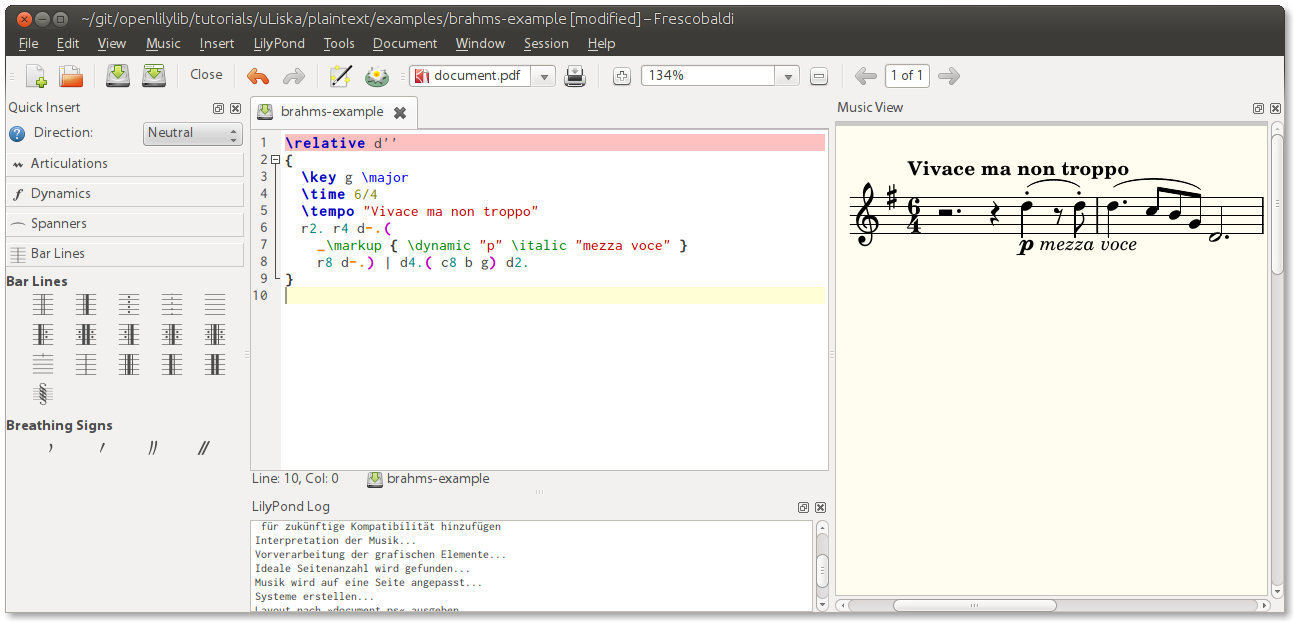
\includegraphics[max width=\textwidth]{examples/frescobaldi/main-window}
\caption{Frescobaldi's Main Window}
\label{fig:pt_fb-main-window}
\end{figure}

Another example of the useful tools is the \emph{Score Setup Wizard} that allows you to graphically configure a score of arbitrary complexity (just like in other programs) and that generates the text used for the corresponding score for you (see \fref{fig:pt_fb-score-setup-wizard}).

\begin{figure}
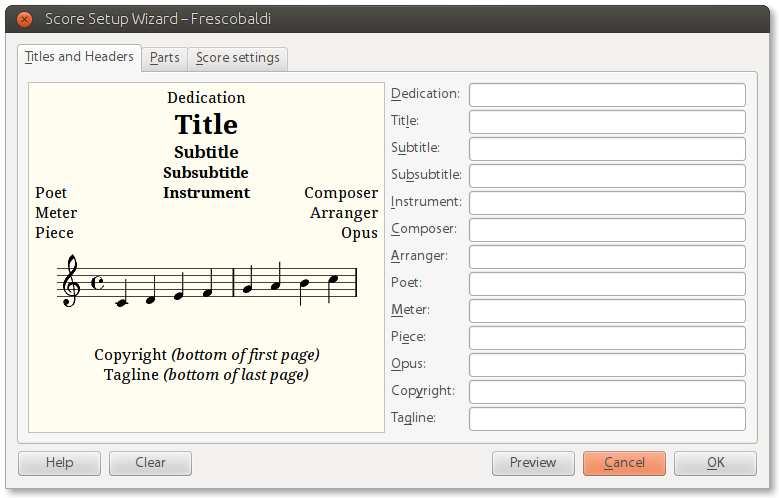
\includegraphics[max width=\textwidth]{examples/frescobaldi/score-wizard}
\caption{Frescobaldi: Score Setup Wizard}
\label{fig:pt_fb-score-setup-wizard}
\end{figure}

If you look at the text editor again (in \fref{fig:pt_fb-main-window}) you will see that the text is colored a lot (I will talk about the actual text soon).
This is a feature that Frescobaldi shares with most programming editors: it “knows” LilyPond's language and highlights the source text according to its structure.
Once one has got used to that practice it greatly eases reading and writing the necessary text files.

When you start typing a command Frescobaldi can also give you suggestions on how to complete them (\fref{fig:pt_fb-code-completion})---also a valuable assistance, not so much because of its time-saving but because it assists you in remembering and efficiently reduces errors.

\begin{figure}
\centering
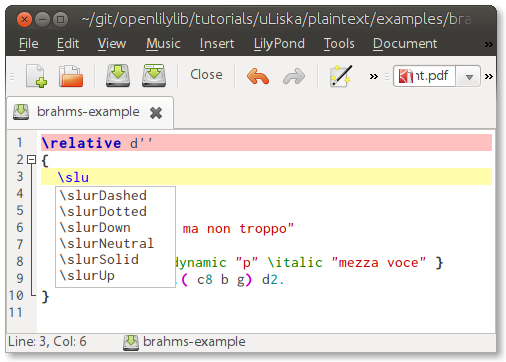
\includegraphics[width=8cm]{examples/frescobaldi/code-completion}
\caption{Frescobaldi: Suggestions for available commands}
\label{fig:pt_fb-code-completion}
\end{figure}

But maybe the most important feature for daily work is that you can click on an element in the music view and will be taken to the corresponding place in the input file.
In \fref{fig:pt_fb-point-and-click} you can see the slur highlighted in purple in the music view and the highlighted text in line 8 in the text editor.
\begin{figure}
\centering
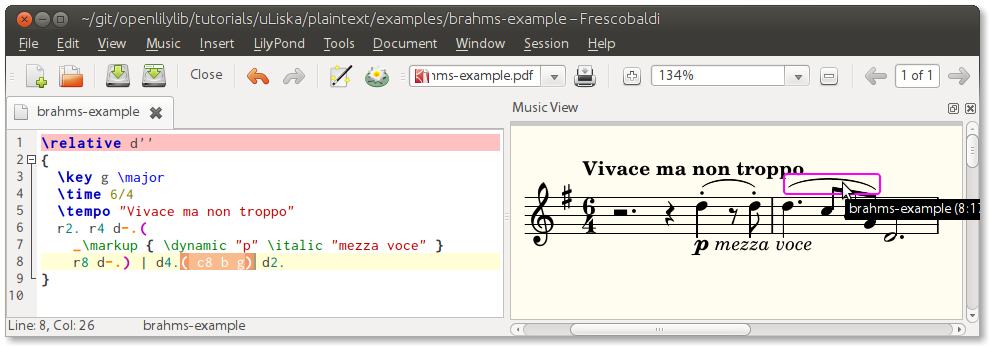
\includegraphics[max width=\textwidth]{examples/frescobaldi/point-and-click}
\caption{Frescobaldi: Two-way link between input file and score}
\label{fig:pt_fb-point-and-click}
\end{figure}
This also works in the other direction: If you select text in the editor the corresponding notation elements are highlighted in the score.
This lets you easily navigate your text file(s) and removes a handicap one could have seen in editing plain text files in the past.

One focus of current Frescobaldi development is the enhancement of the music view's functionality.
So it will soon be possible to partially “edit” the score with the mouse---of course in fact you will be able to tweak something visually and Frescobaldi will insert the appropriate text in the source file, possibly giving you the option to select from different approaches.
Currently there are plans to implement (e.\,g.) correcting pitches, drawing and shaping curves, and annotating objects (see also \fref{sec:pt_lilypond-comments}).
This will make “working with text files” even more comfortable.

Of course these remarks were only a very cursory overview of Frescobaldi.
A thorough introduction can't be the intention of this paper, but I wanted to give you a feeling to what extent current and smart editors can smoothen your editing experience.
Now you are ready to learn something about how LilyPond input files actually work.

\section{Textual Representation of Music}
\label{sec:pt_textual-representation}
In \fref{fig:pt_fb-main-window} (and \fref{fig:pt_fb-point-and-click}) you have seen a short score excerpt from Brahms' first violin sonata, along with the LilyPond code that produced it.
Now I'll use that example to show you a little bit about the basic elements in a LilyPond score.

At the most basic level notes are represented by their pitch and duration, as you can see in this “bare” example:

\begin{multicols}{2}
\begin{Verbatim}[samepage=true,
				   commandchars=|„“]
{
  r2. r4 d r8 d
  d4. c8 b g d2.
}
\end{Verbatim}
\columnbreak
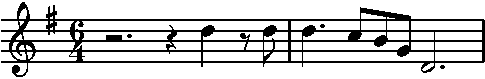
\includegraphics{examples/brahms/brahms-1}
\end{multicols}

The text writes rests (\texttt{\textit{r}}) and pitches (\texttt{\textit{d}} etc.), and everything is enclosed in a pair of curly braces.
This is LilyPond's notion of a \emph{music expression}.
A score is represented by one big music expression which can be constructed of arbitrarily nested smaller music expressions.
There are a few things “missing” in the source that LilyPond adds by itself, namely a staff, a clef, and beams.

Two more elements aren't actually figured out automatically, but hidden from the example.
In fact you have to write down \cmd{key g} \cmd{major} and \cmd{time 6/4} to tell LilyPond about the key and time signatures.
But the beaming in the second measure is done automatically according to the time signature.
Many things can be defined by such \emph{commands}.

Elements like articulations or dynamics are attached to notes or rests by printing them after the reference item, like in this fake example:

\newcommand{\hilite}[1]{\textcolor{red}{\textbf{#1}}}

\begin{multicols}{2}
\begin{Verbatim}[samepage=true,
				   commandchars=|„“]
{
  r2. r4 d|hilite„-.“ r8 d|hilite„-.“ 
  d4.|hilite„\sf“ c8|hilite„\>“ b g|hilite„\!“ d2.|hilite„->“
}
\end{Verbatim}
\columnbreak
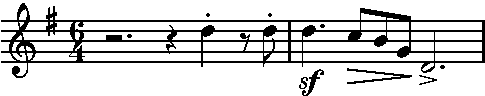
\includegraphics{examples/brahms/brahms-2}
\end{multicols}

We have a few articulations that are attached with a hyphen, the staccato dot written as a dot, the accent as a \texttt{>}, all characters have been chosen to be as intuitive as possible.
Dynamics are attached by a backslash, in the example we have the \lilyDynamics{sf} with \cmd{sf}, the \decrescHairpin with \cmd{>}, and (as the only unusual item) the \cmd{!} which represents the \emph{end} of the hairpin.

We can attach \emph{spanners} to pairs of notes, e.\,g.\ the slur in the first measure of the following example.
Slurs are written as opening and closing round brackets (\emph{after} the note they are referring to)
There you can see that you can attach multiple items to a note by just writing them one after another

\begin{multicols}{2}
\begin{Verbatim}[samepage=true,
				   commandchars=|„“]
{
  r2. r4 d-.|hilite„(“ r8 d-.|hilite„)“
  d4.|hilite„(“ c8|hilite„[“ b|hilite„]“ g|hilite„)“ d2.
}
\end{Verbatim}
\columnbreak
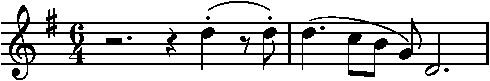
\includegraphics{examples/brahms/brahms-3}
\end{multicols}

In addition to the slurs you can also see an example of manually setting the beams against the rules for the time signature, which is indicated by the use of square brackets (again \emph{after} the notes they are referring to).

In the last example of this \emph{very} short introduction to LilyPond files we'll add the necessary text elements to the score.
The \emph{tempo} indication is entered by the \cmd{tempo} command (the non-verbal part is here as an example only), while the \lilyDynamics{p} \emph{mezza voce} is a \cmd{markup}---a text that is attached to a note like any articulation or dynamic sign.

\begin{multicols}{2}
\begin{Verbatim}[samepage=true,
				   commandchars=|„“]
{
  |hilite„\tempo“ "Vivace ma non troppo" |hilite„2. = 60“
  r2. r4 d-.(|hilite„-\markup“
    { \dynamic "p" \italic "mezza voce" } 
    r8 d-.) 
  d4.( c8 b g) d2.
}
\end{Verbatim}
\columnbreak
\vspace*{4.5em}
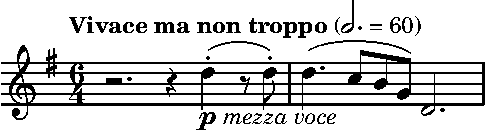
\includegraphics{examples/brahms/brahms-4}
\end{multicols}

One thing you may have noticed in the example is that I have broken the first line of music into three.
LilyPond doesn't care about this \emph{white space} and allows you to lay out your text file as you find appropriate---which usually will mean to keep coherent entities on a single line.
In this case the entity is the \emph{markup}, also an expression enclosed in curly braces.
You could just throw some text in there, but in this score we format the elements, one using the dynamics font, the other as italic text.

\medskip
Now you've seen your first real-world example of a LilyPond score.
Of course the complexity of these text files increases when the music gets longer or more complex.
But when looking at an input file you should always keep in mind that it is built from very small and rather simple units.
And you should feel comfortable with knowing that there are editors at hand that really help you navigating and improving them.

\section{Variables and Includes}
\label{sec:pt_variables-includes}

\section{Comments}
\label{sec:pt_lilypond-comments}



\chapter{\LaTeX}
\label{chap:pt_latex}

\chapter{Applications}
\label{chap:pt_applications}

\section{Single-source Publishing}
\label{sec:pt_single-source-publishing}

\chapter{Where To Go From Here?}
\label{chap:pt_where-to-go-from-here}

\begin{itemize}
\item Recommended introductory material for all aspects
\end{itemize}
\end{document}